\chapter{2D Systems}\label{ch:2Dsyst}



In this work, it is mainly used to model a simplified body in papers...


Rectangular system described by state variable $u = u(x,y,t)$  where $t\geq 0$ and $(x,y) \in \D$ where $\D$ is 2-dimensional. The state variable can then be discretised according to $u(x, y, t) \approx \ulmn$ with space $x = lh$ and $y = mh$ and time $t = nk$ and $k=1/\fs$. For simplicity, this work assumes the grid spacing in both the $x$ and $y$ directions are set to be the same.

Circular or elliptical systems can be modelled using a staircase approximation or radial coordinates \cite{theBible}. 

In continuous time the  operators:
\begin{equation}\label{eq:laplacian}
    \Delta = \pxx + \pyy
\end{equation}


The same shift operators as defined in Chapter \ref{ch:FDTD} can be applied to grid function $\ulmn$. Additional ones are
\begin{equation}
    e_{y+}\ulmn = u_{l, m+1}^n,\quad \text{and}\quad e_{y-}\ulmn= u_{l, m-1}^n.
\end{equation}

\section{Analysis Techniques in 2D}\label{sec:analysis2D}
Here, some of the differences between the analysis techniques presented in Chapter \ref{ch:analysis} and those in 2D will be elaborated on. Although, modal analysis remains the same

\subsection{Frequency Domain Analysis}
$p_x + p_y$

ansatz:
\begin{equation}
    \ulmn = z^n e^{jh(l\beta_x + m\beta_y)}
\end{equation}


\subsection{Modal Analysis}
Stacked matrix form

\section{2D Wave Equation}
The 2D wave equation be used to model an ideal membrane such as done in 

It has identical behaviour to the 2D waveguide mesh presented by van Duyne and Smith \cite{Duyne1993}.

This section will present the 2D wave equation in continuous time and discretise it afterwards. Then it will be used as a test-case to explain the various analysis techniques presented in Chapter \ref{ch:analysis} in 2D and the differences with 1D highlighted.

\subsection{Continuous time}
Consider a square ideal membrane with side lengths $L_x$ and $L_y$ (both in m) and its transverse displacement described by $u = u(x,y,t)$. The membrane is defined over $(x,y) \in \D$ with domain $\D = [0, L_x] \times[0, L_y]$ and its motion is described by the following PDE
\begin{equation}\label{eq:2DwavePDE}
    \ptt u = c^2\Delta u
\end{equation}
with wave speed $c = \sqrt{T/\rho H}$ (in m/s), tension per unit length (applied to the boundary)\todo{check whether this is right..}$T$ (in N/m), material density $\rho$ (in kg/m$^3$) and thickness $H$.



\subsection{Energy Analysis in 2D}
Analogous to the continuous 2D domain $\D$, one can define a 2D discrete domain $d\in \{0, \hdots, N_x\} \times \{0, \hdots, N_y\}$
\begin{equation}\label{eq:2DInnerProd}
    \langle f^n_{l, m}, g^n_{l, m} \rangle_d = \sum_{l = 0}^{N_x}\sum_{m = 0}^{N_y} h^2 f_{l,m}^n g_{l,m}^n
\end{equation}

Reduced domains are defined as $\underline{d} = \{0, \hdots, N_x-1\} \times \{0, \hdots, N_y-1\}$ and $\underline{\overline{d}} = \{1, \hdots, N_x-1\}\times\{1, \hdots, N_y-1\}$.

\section{Thin plate}\label{sec:thinPlate}
Used in \citeP[A], \citeP[B], \citeP[D] and \citeP[E]
biharmonic operator, Laplacian in \eqref{eq:laplacian} applied to itself.
\begin{equation}\label{eq:platePDENoLosses}
    \rho H \ptt u = -D\Delta\Delta u
\end{equation}
where $D = EH^3/12(1-\nu^2)$.

Adding losses to \eqref{eq:platePDE} yields 

\begin{equation}\label{eq:platePDE}
    \rho H \ptt u = -D\Delta\Delta u - 2\sz \rho H \pt u + 2 \so\rho H  \pt \Delta u
\end{equation}

\begin{equation}\label{eq:plateUpdate}
    \ulm^{n+1}
\end{equation}

\def\figSpacing{0.01\textwidth}
\def\figWidth{0.49\textwidth}

\begin{figure}[t]
    \centering
    \subfloat[Full stencil.\label{fig:fullStencilPlate}]{\includegraphics[width=\figWidth]{figures/resonators/2d/fullPlate.eps}}\\
    \subfloat[Stencil of $u_{l,m}^n$. \label{fig:curStencilPlate}]{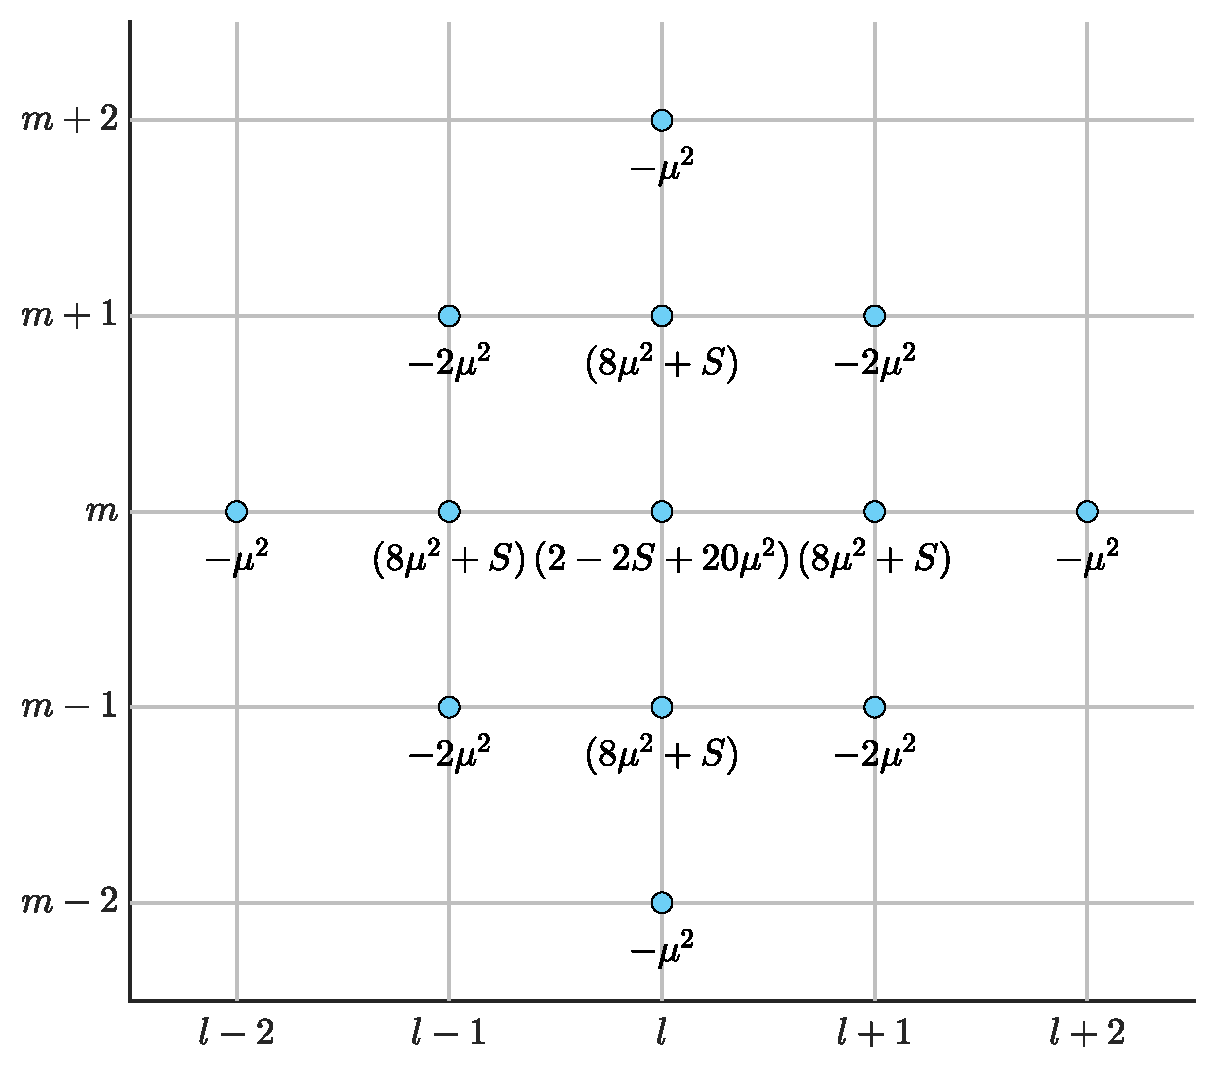
\includegraphics[width=\figWidth]{figures/resonators/2d/curPlateStencil.eps}}\hspace{\figSpacing}
    \subfloat[Stencil of $u_{l,m}^{n-1}$.\label{fig:prevStencilPlate}]{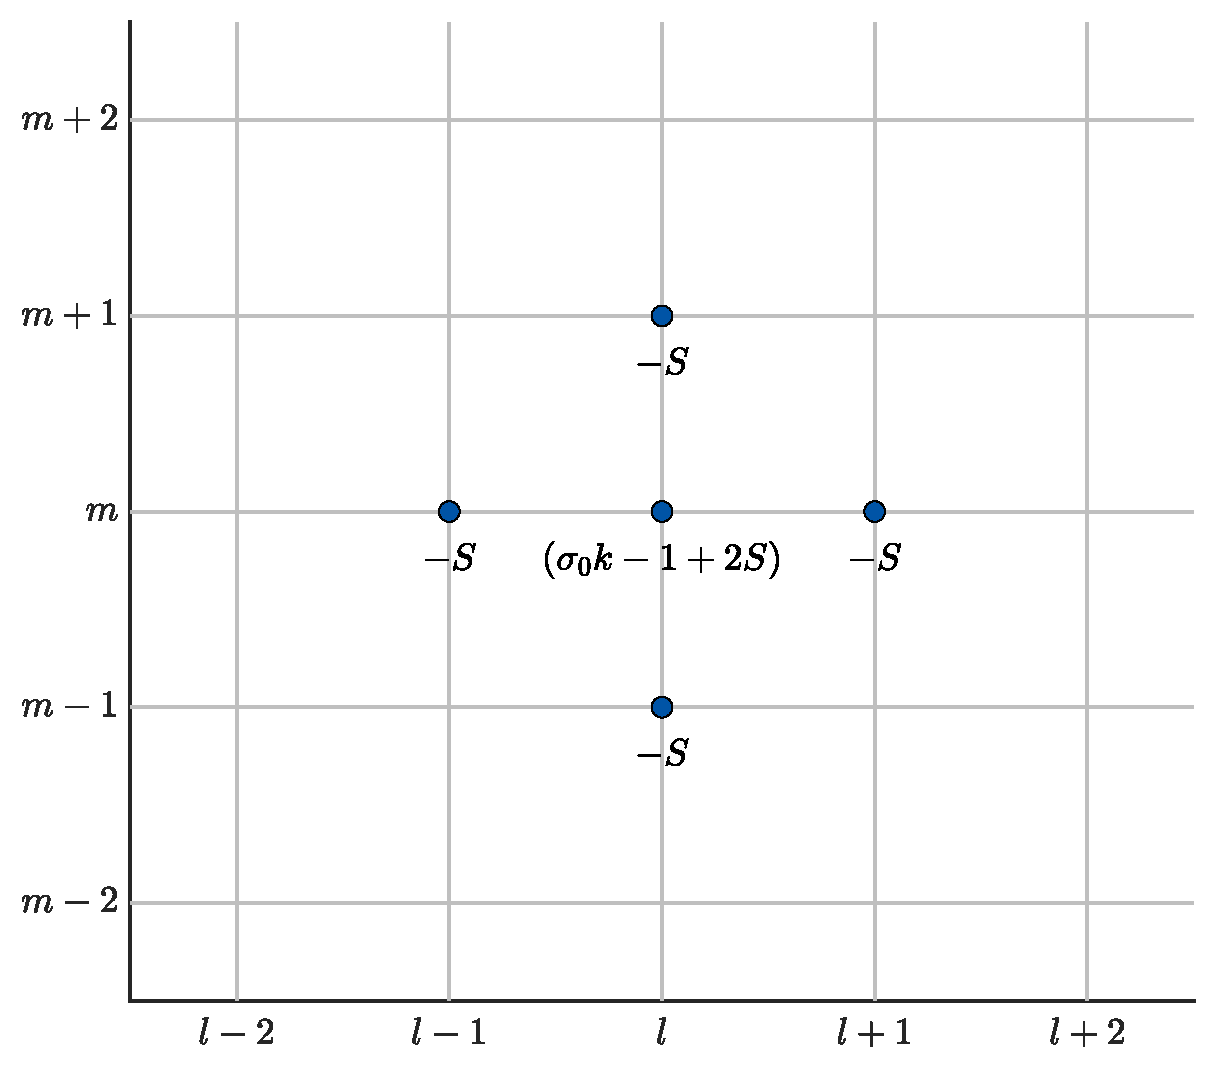
\includegraphics[width=\figWidth]{figures/resonators/2d/prevPlateStencil.eps}}
    \caption{The stencil of the plate with various parts of update equation \eqref{eq:plateUpdate} shown (using $S = 2\so k/h^2$ for brevity). (a) An overview. (b) The current time-step $n$. (c) The previous time-step $n-1$. \label{fig:plateStencil}}
\end{figure}

\subsection{Energy Analysis}
\begin{equation}
    \dtp \h = -\q 
\end{equation}
where 
\begin{equation}\label{eq:energyBalanceThinPlate}
    \begin{gathered}
        \h = \t + \v, \qwiq \t = \frac{\rho H}{2} \left\lVert\delta_{t-}\ulmn\right\rVert_{d}^2 \quad \text{and} \\
        \v = \frac{D}{2}\langle\delta_{\Delta\boxplus} \ulmn, e_{t-}\delta_{\Delta\boxplus} \ulmn\rangle_{\overline{\underline{d}}}\ .
    \end{gathered}
\end{equation}
and 
\begin{equation}\label{eq:dampingTermThinPlate}
    \mathfrak{q} = 2\sz \rho A \lVert\dtd\ulmn\rVert_d^2 - 2 \so \rho A \langle \dtd \ulmn, \dtm \delta_{\Delta\boxplus}\uln \rangle_d,
\end{equation}

\section{Stiff membrane}
Like the stiff string, the membrane can be extended with a stiffness term to yield a \textit{stiff membrane} \cite{Fletcher1998}. This model has been used for paper \citeP[F]...
Combining between Eqs. \eqref{eq:2DwavePDE} and \eqref{eq:platePDE} including the losses yields
\begin{equation}\label{eq:stiffMembrane}
    \rho H \ptt u = T\Delta u - D
    \Delta\Delta u
\end{equation}


Is essentially a 2D stiff string. 